% Author: Izaak Neutelings (October 2020)
\documentclass[border=3pt,tikz]{standalone}
\usepackage{physics}
\usepackage{tikz}
\usepackage[outline]{contour} % glow around text
\usetikzlibrary{calc}
\usetikzlibrary{angles,quotes} % for pic
\usetikzlibrary{arrows.meta}
\usetikzlibrary{patterns}
\tikzset{>=latex} % for LaTeX arrow head
\contourlength{1.35pt}

\colorlet{xcol}{blue!70!black}
\colorlet{vcol}{green!60!black}
\colorlet{myred}{red!65!black}
\colorlet{mypurple}{blue!60!red!80}
\colorlet{acol}{red!50!blue!80!black!80}
\tikzstyle{rvec}=[->,xcol,very thick,line cap=round]
\tikzstyle{vvec}=[->,vcol,very thick,line cap=round]
\tikzstyle{myarr}=[{Latex[length=3,width=3]}-,xcol]
\tikzstyle{force}=[->,myred,very thick,line cap=round]
\tikzstyle{Fproj}=[force,myred!40]
\tikzstyle{mass}=[line width=0.6,draw=red!30!black, %rounded corners=1,
                  top color=red!40!black!30,bottom color=red!40!black!10,shading angle=30]
\tikzstyle{ground}=[preaction={fill,top color=black!10,bottom color=black!5,shading angle=20},
                    fill,pattern=north east lines,draw=none,minimum width=0.3,minimum height=0.6]
\tikzstyle{metal}=[fill,top color=black!40,bottom color=black!20,shading angle=10]


\def\r{0.05} % pulley small radius
\tikzset{
  pics/Tin/.style={
    code={
      \def\R{0.12}
      \draw[pic actions,line width=0.6,#1,fill=white] % ,thick
        (0,0) circle (\R) (-135:.75*\R) -- (45:.75*\R) (-45:.75*\R) -- (135:.75*\R);
  }},
  pics/Tout/.style={
    code={
      \def\R{0.12}
      \draw[pic actions,line width=0.6,#1,fill=white] (0,0) circle (\R);
      \fill[pic actions,#1] (0,0) circle (0.3*\R);
  }},
  pics/Tin/.default=mypurple,
  pics/Tout/.default=mypurple,
}

\begin{document}


% ROLLING
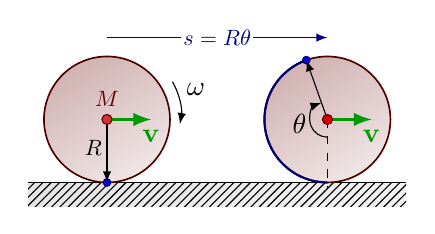
\begin{tikzpicture}
  \def\W{4.8} % ground width
  \def\H{3.2} % ground height
  \def\D{0.3} % ground depth
  \def\R{0.8} % disk radius
  \def\d{1.0} % disks' distances from edge
  \def\angb{{(2*\d-\W)*180/pi-90}} % angle point 2
  \coordinate (A)  at (\d,\R);     % disk 1 origin
  \coordinate (B)  at (\W-\d,\R);  % disk 2 origin
  \coordinate (RA) at ($(A)+(-90:\R)$);   % point 1
  \coordinate (RB) at ($(B)+(\angb:\R)$); % point 2
  \coordinate (BB) at ($(B)+(-90:\R)$);   % point 2 bottom
  
  % GROUND
  \draw[ground] %(0,0) rectangle++ (-\D,\H) (-\D,\H) rectangle++ (\W,\D);
    (0,0) rectangle++ (\W,-\D);
  \draw (0,0) --++ (\W,0);
  
  % DISK 1
  \draw[mass] (A) circle(\R);
  \draw[blue!50!black,fill=blue!90!black] (RA) circle(0.06*\R);
  \draw[->] (A) -- (RA) node[midway,above=1,left=-1,scale=0.8] {$R$}; %node[right=3] {$M$}
  \draw[vvec] (A) --++ (0.7*\R,0) node[below] {$\vb{v}$};
  \draw[red!40!black,fill=red!80!black!80] (A) circle(0.08*\R) node[above=2,scale=0.8] {$M$}; %node[right=1,scale=0.8] {CM}
  %\draw[force] (TD)++(0.08,0) --++ (0,0.8*\RD) node[right] {$\vb{T}$};
  \draw[->] (A)++(30:1.2*\R) arc(30:-10:1.0*\R) node[midway,above right=-1] {$\omega$};
  
  % DISK 2
  \draw[mass] (B) circle(\R);
  \draw[thick,blue!40!black] (BB) arc(-90:\angb:\R);
  \draw[blue!50!black,fill=blue!90!black] (RB) circle(0.06*\R);
  \draw[->] (B) -- (RB);
  \draw[dashed] (B) --++ (0,-\R) --++ (0,-0.1*\R);
  \draw[vvec] (B) --++ (0.7*\R,0) node[below] {$\vb{v}$};
  \draw[red!40!black,fill=red!80!black] (B) circle(0.08*\R);
  \draw pic[<-,scale=0.8,"$\theta$",draw,angle radius=8,angle eccentricity=1.6] {angle=RB--B--BB};
  \draw[->,blue!50!black] (A)++(0,1.3*\R) --++ (\W-2*\d,0) node[midway,fill=white,inner sep=1,scale=0.8] {$s=R\theta$};
  %\draw[->] (B)++(30:1.2*\R) arc(30:-10:1.0*\R) node[midway,above right=-1] {$\omega$};
  
\end{tikzpicture}



% INCLINED ground
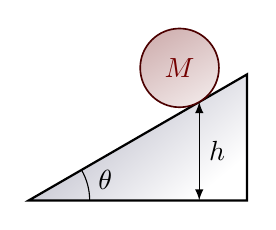
\begin{tikzpicture}
  \def\R{0.5} % disk radius
  \def\W{3.2}  % ground width
  \def\ang{30} % ground angle
  \def\mx{2.5} % mass x position
  \coordinate (X) at (\ang:\mx); % wheel position
  \coordinate (C) at ($(X)+(\ang+90:\R)$); % wheel center
  \draw[thick,top color=blue!20!black!30,bottom color=white,shading angle=\ang+10]
    (0,0) coordinate (O) -- (\ang:\W) coordinate (T) -- ({\W*cos(\ang)},0) coordinate (L) -- cycle;
  \draw[mass] (C) circle(\R) node[myred!70!black] {$M$};
  \draw pic["$\theta$",draw=black,angle radius=22,angle eccentricity=1.3] {angle=L--O--T};
  \draw[<->] (X) --++ (0,{-\mx*sin(\ang)}) node[midway,right] {$h$};
\end{tikzpicture}



\end{document}
